%%%%%%%%%%%%%%%%%%%%%%%%%%%%%%%%%%%%%%%%
%% MCM/ICM LaTeX Template %%
%% 2020 MCM/ICM           %%
%%%%%%%%%%%%%%%%%%%%%%%%%%%%%%%%%%%%%%%%
\documentclass[12pt]{article}
% \documentclass{article}
\usepackage{geometry}
\geometry{left=1in,right=0.75in,top=1in,bottom=1in}

%%%%%%%%%%%%%%%%%%%%%%%%%%%%%%%%%%%%%%%%
% Replace ABCDEF in the next line with your chosen problem
% and replace 1111111 with your Team Control Number
\newcommand{\Problem}{\textcolor{cyan}{REPLACE ME WITH PROBELM}}
\newcommand{\Team}{\textcolor{cyan}{REPLACE ME WITH TEAM NUMBER}}
%%%%%%%%%%%%%%%%%%%%%%%%%%%%%%%%%%%%%%%%

% \usepackage{newtxtext}
\usepackage{amsmath,amssymb,amsthm}
\usepackage{newtxmath} % must come after amsXXX

\usepackage[pdftex]{graphicx}
\usepackage{xcolor}
\usepackage{fancyhdr}
\usepackage{setspace}
\usepackage{amsmath}
\usepackage{graphicx}
\usepackage{float}
\usepackage{subcaption}
% This is gonna give you footnote
% \usepackage[backend=bibtex,style=verbose-trad2]{biblatex}
% And this is gonna give you some collection
\usepackage[backend=bibtex,style=ieee]{biblatex}
\usepackage{siunitx} % Required for alignment
\usepackage{multirow}
\usepackage{booktabs} % For prettier tables
\usepackage{longtable} % To display tables on several pages
\usepackage{rotating} % To display tables in landscape
\usepackage{pgfplotstable} % Generates table from .csv
\usepackage{tikz}
\usepackage{pgfplots}
\usepackage{csvsimple}
\usepackage{listings}
\usepackage[utf8]{inputenc}
% Well guess you need this to make sure line break of minted listing is working fine
\usepackage[newfloat]{minted}
% \usepackage{caption}
\usepackage{pgf}
\usepackage{import}
\usepackage{pdfpages}
\bibliography{summary}


\lhead{Team \Team}
\rhead{}
\cfoot{}

\newtheorem{theorem}{Theorem}
\newtheorem{corollary}[theorem]{Corollary}
\newtheorem{lemma}[theorem]{Lemma}
\newtheorem{definition}{Definition}

%%%%%%%%%%%%%%%%%%%%%%%%%%%%%%%%
\begin{document}
\graphicspath{{.}}  % Place your graphic files in the same directory as your main document
\DeclareGraphicsExtensions{.pdf, .jpg, .tif, .png}
\thispagestyle{empty}
\vspace*{-16ex}
\centerline{\begin{tabular}{*3{c}}
        \parbox[t]{0.3\linewidth}{\begin{center}\textbf{Problem Chosen}\\ \Large \textcolor{red}{\Problem}\end{center}}
         & \parbox[t]{0.3\linewidth}{\begin{center}\textbf{2020\\ MCM/ICM\\ Summary Sheet}\end{center}}
         & \parbox[t]{0.3\linewidth}{\begin{center}\textbf{Team Control Number}\\ \Large \textcolor{red}{\Team}\end{center}} \\
        \hline
    \end{tabular}}
%%%%%%%%%%% Begin Summary %%%%%%%%%%%
% Enter your summary here replacing the (red) text
% Replace the text from here ...
\begin{center}
    \textcolor{red}{%
        Use this template to begin typing the first page (summary page) of your electronic report. This \newline
        template uses a 12-point Times New Roman font. Submit your paper as an Adobe PDF \newline
        electronic file (e.g. 1111111.pdf), typed in English, with a readable font of at least 12-point type.	\\[2ex]
        Do not include the name of your school, advisor, or team members on this or any page.	\\[2ex]
        Papers must be within the page limit specified in the problem statement.	\\[2ex]
        Be sure to change the control number and problem choice above.	\\
        You may delete these instructions as you begin to type your report here. 	\\[2ex]
        \textbf{Follow us @COMAPMath on Twitter or COMAPCHINAOFFICIAL on Weibo for the \newline
            most up to date contest information.}
    }
\end{center}
% to here
%%%%%%%%%%% End Summary %%%%%%%%%%%

%%%%%%%%%%%%%%%%%%%%%%%%%%%%%%
\clearpage
\pagestyle{fancy}
% Uncomment the next line to generate a Table of Contents


\begin{center}
    \Large \textbf{Kingdom Built on a Pile of Sand:Slow and Steady}
\end{center}

\newpage

\tableofcontents
\newpage
\setcounter{page}{1}
\rhead{Page \thepage\ }

\section{Introduction}
\subsection{Problem Background}
Sunshine, clear blue sea and golden color sand always seem to leave people in a happy state of mind.
And a beach is where these three are combined, drawing people all around towards it. Sand, the granular matter formed by constant brushing of flowing water, however, can react with water in a different way, despite the fact that people refer to it as non-stable or unreliable. On a beach, where the already formed granular sand and the rise and fall of sea wave lies together, a new buff can be added to our flowing friend, a wetted state.
\par
Magically but not randomly, sand gets sticky when combined with water, due to the most obvious physical theorem: surface tension and atmosphere pressure. From previous people's work, we've know that this buff comes from the water bridge formed between sand particles, which can significantly cluster together during the increasing water-sand portion\autocite{pakpour2012construct,mitarai2006wet,kudrolli2008sticky}. Kudrolli and Arshad has visualized the bridge between sand like Figure \ref{fig:water_bridge}.
\par
And that's the magic that glue our favorite sand castle together, which is one of the most entertainment for enthusiastic beach goers. However, being built near the water that melts mud and our wet sand, all sand castles have to face the fate that they'll g et too wet to hold its own weight and the impact from sea waves. That's because the water bridge has another property of clustering together\autocite{kudrolli2008sticky}. When you throw a pile of sand into water, they behave just as when they're completely dry, melting down like fluid. Thus beach castle builder might want to make their sand castle last longer than those build arbitrarily than others, which is also the purpose of this article. 


\begin{figure}
    \centering
    \includegraphics[width=0.5\linewidth]{water_bridge.eps}
    \caption{Water Bridge Between Sand Particle}
    \label{fig:water_bridge}
\end{figure}

\subsection{Our Work}
Normally people will sculpt their kingdom from a pile of tedious wet sand. To simplify the model and grasp main threads, we'll focus our research on this single, nondescriptive mound of wetted sand.

\section{Assumptions \& Nomenclature}
\subsection{Assumptions}
\subsection{Nomenclature}


\section{Modeling Under Waves and Tides}

\textcolor{cyan}{This is a test figure. Remember to delete me.}
\begin{figure}[H]
    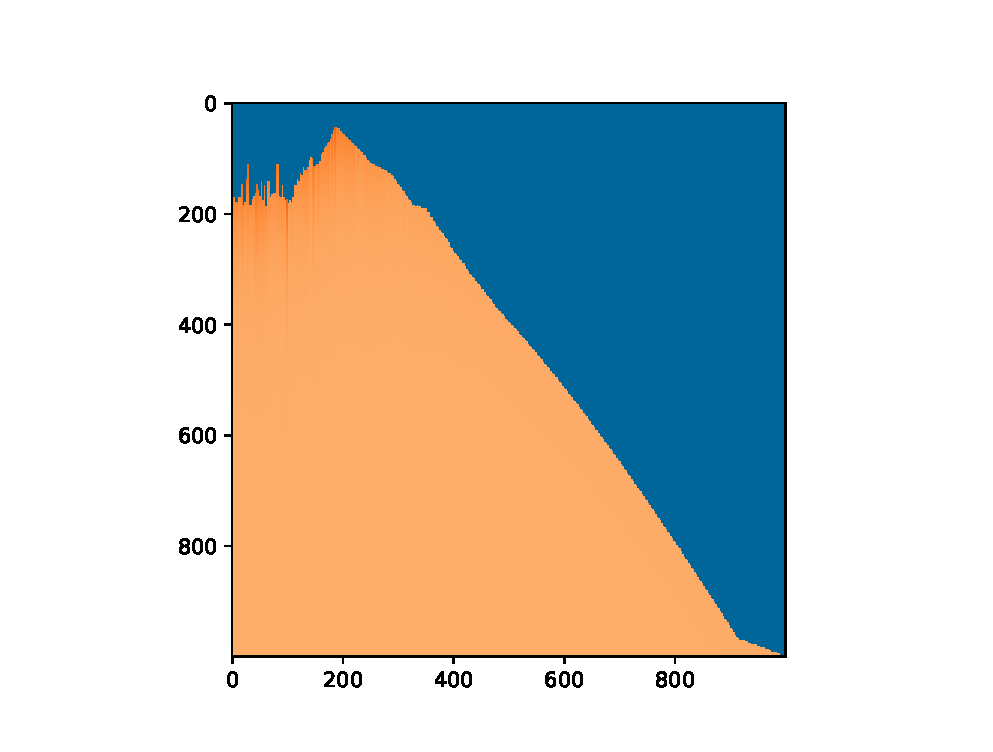
\includegraphics[width=\linewidth]{Figure_1.eps}
    \caption{A Windows Terminal.}
    \label{fig:Terminal}
\end{figure}
\textcolor{cyan}{This is a test figure. Remember to delete me.}
\begin{figure}[H]
    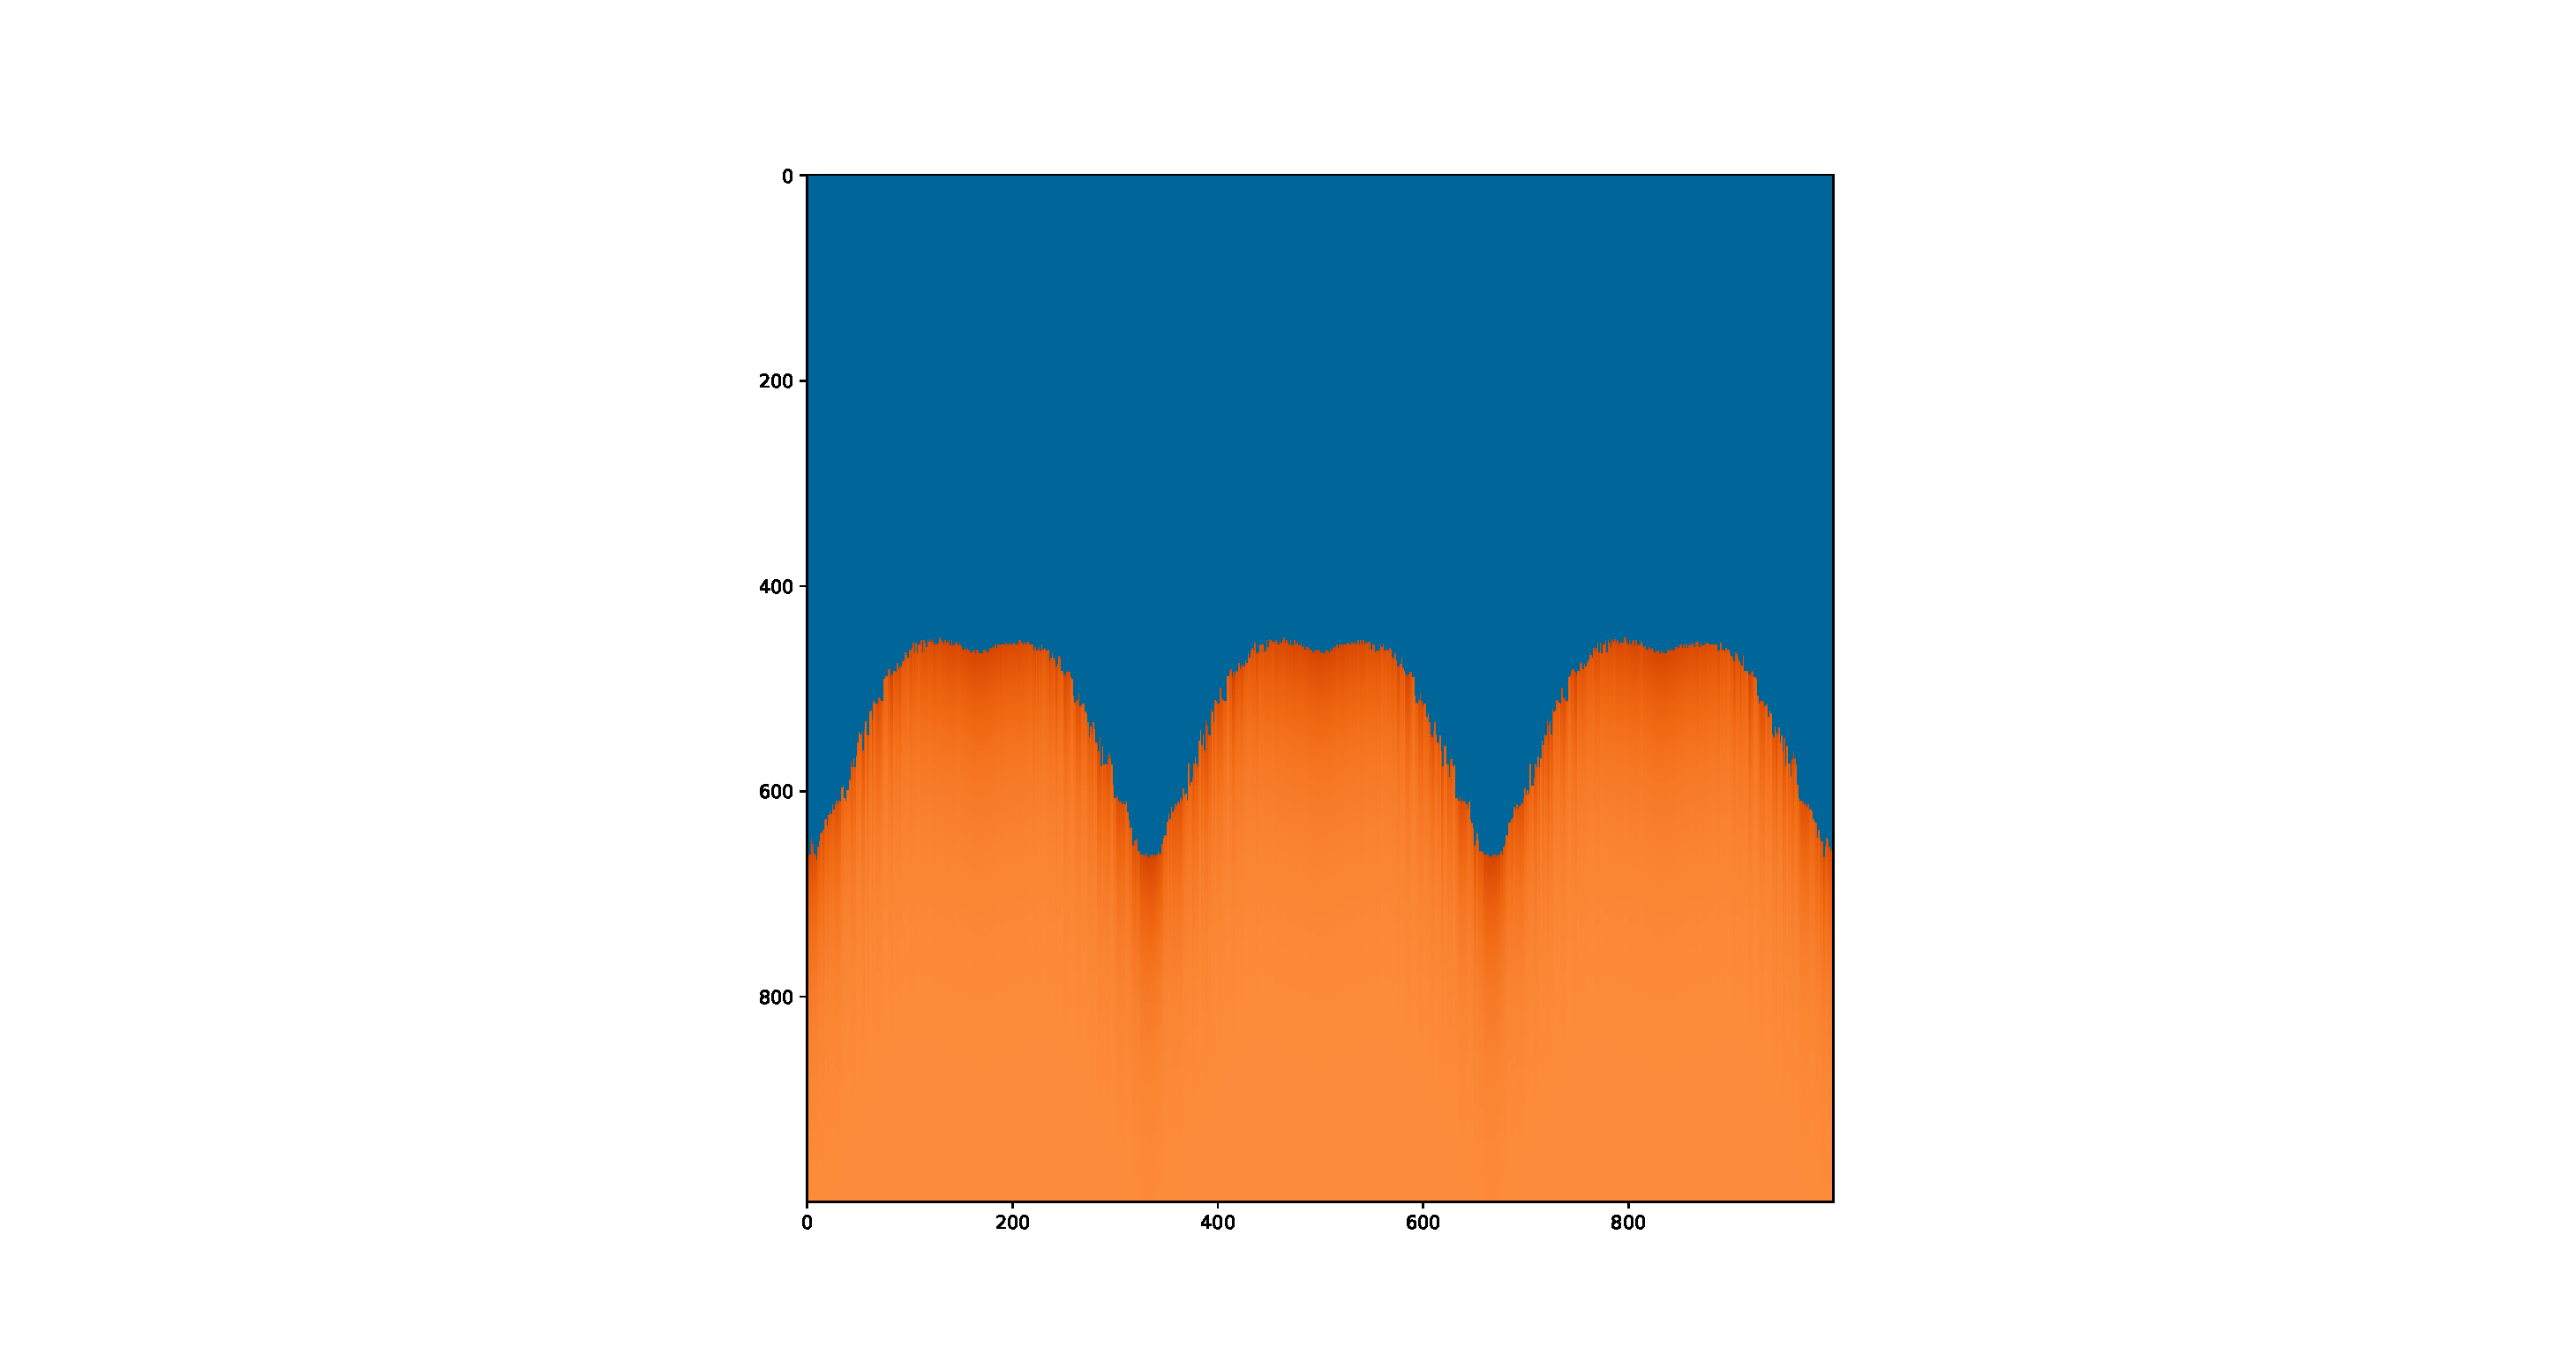
\includegraphics[width=\linewidth]{Figure_2.eps}
    \caption{A Windows Terminal.}
    \label{fig:Terminal}
\end{figure}

\subsection{Shape of the Slope: Mohr-Coulomb Criterion}


\subsection{Top View Shape}
\subsection{Calculating Results}
\subsection{Simulating Results}
This is some example text\footnote{\label{myfootnote}Hello footnote}.

I'm referring to footnote \ref{myfootnote}.

\section{Modeling Under Rain}

\section{Determine the Best Sand-to-water Proportion}

\section{Other Ways to Make Our Sand Castle Last Longer}

\section{Sensitivity Analysis}

\newpage
\begin{appendix}
    \listoffigures
    \listoftables
    \listoflistings
    % \bibliographystyle{ieeetr}
    \printbibliography
\end{appendix}
\end{document}
